\documentclass[preprint]{aastex631}
\usepackage{verbatim, placeins}

\newcommand{\HL}[1]{\textcolor{red}{\bf#1}}
\newcommand{\num}[1]{\textcolor{cyan}{\bf#1}}

\newcommand{\minimize}{$\texttt{SciPy.optimize.minimize()}$}
\newcommand{\neldarmead}{\texttt{Nelder-Mead}} 
\newcommand{\newtoncg}{\texttt{Newton-CG}}
\newcommand{\bfgs}{\texttt{BFGS}}
\newcommand{\sfit}{\texttt{SFit}}

\begin{document}

\title{An Alternate Method for Minimizing $\chi^2$}

\author{Jennifer C. Yee}
\author{Andrew P. Gould}

\begin{abstract}
In this paper, we describe an algorithm and associated software package (\texttt{sfit\_minimize}) for maximizing the likelihood function of a set of parameters by minimizing $\chi^2$. The key element of this method is that the algorithm estimates the second derivative of the $\chi^2$ function using first derivatives of the function to be fitted. These same derivatives can also be used to calculate the uncertainties in each parameter. We test this algorithm against several standard minimization algorithms in \minimize\, by fitting point lens models to light curves from the 2018 Korea Microlensing Telescope Network event database. We show that for fitting microlensing events, \sfit\, works faster than the \neldarmead\, simplex method and is more reliable than the \bfgs\, gradient method.
\end{abstract}

\section{The Derivation}

Our method builds upon the discussion in ``$\chi^2$ and Linear Fits" \citep{Gould03}, which noted that the approach to non-linear models could be expanded beyond the scope of that work. Suppose that the function we want to minimize is a function $F(x)$ that is described by $n$ parameters $A_i$ (where we use $A_i $ (instead of $a_i$) as a reminder that in the general
case, they are non-linear). Considering
the general (nonlinear) case, we can Taylor expand $\chi^2$, in terms of the $n$ parameters:
\begin{eqnarray}
\chi^2 & = &  \chi^2_0 + \sum_i {\partial \chi^2\over \partial A_i} A_i
+ {1\over2}\sum_{i,j} {\partial^2 \chi^2\over \partial A_i \partial A_j}A_i A_j\\
& = & \chi^2_0 + \sum_i D_i * A_i + \sum_{i,j} B_{ij} * A_i A_j  + ... \quad,
\end{eqnarray}
where
\begin{eqnarray}
D_i  & \equiv & {\partial \chi^2\over \partial A_i} \label{eqn:d}\\
B_{ij} & \equiv & (1/2){\partial^2 \chi^2\over \partial A_i\partial A_j}  \quad. \label{eqn:b}
\end{eqnarray}
Then,
\begin{equation}
\frac{\partial \chi^2}{\partial A_i} = -2\sum_k \frac{(y_k - F(x_k))}{\sigma^2_k}\frac{\partial F(x_k)}{\partial A_i}
\end{equation}
and
\begin{equation}
\frac{\partial^2 \chi^2}{\partial A_i \partial A_j} = -2\sum_k \left[
 \frac{1}{\sigma^2_k}\frac{\partial F(x_k)}{\partial A_i}\frac{\partial F(x_k)}{\partial A_j} +
  \frac{(y_k - F(x_k))}{\sigma^2_k}\frac{\partial^2 F(x_k)}{\partial A_i \partial A_j}
 \right] \quad .
\end{equation}
In the special case of a linear function, $F(x) = \sum_i a_i f_i(x)$
then
\begin{equation}
\frac{\partial F(x)}{\partial a_i} = f_i(x)
\quad \mathrm{and} \quad
\frac{\partial^2 F(x)}{\partial a_i\partial a_j} = 0,
\end{equation}
so the second term disappears, and we find that the solution (derived from
second derivative of $\chi^2$) can be expressed
in terms of products of the FIRST derivatives of the general functional
form.  For the general case, we simply make the approximation that the second derivative term can be neglected; i.e.,
\begin{equation}
\frac{\partial^2 \chi^2}{\partial A_i \partial A_j} \approx -2\sum_k 
 \frac{1}{\sigma^2_k}\frac{\partial F(x_k)}{\partial A_i}\frac{\partial F(x_k)}{\partial A_j} \quad.
\end{equation}

Hence, there are three ways to generalize Newton's method (actually discovered by Simpson)
to multiple dimensions:
\begin{enumerate}
\item{Use only first derivatives of the $\chi^2$ function (which is what Simpson did in
   1-D), the so-called gradient method.}
\item{Taylor expand $\chi^2$ and truncate at second term, then
   solve this (very inexact equation) exactly by inversion
   of the matrix of second derivatives (Hessian).}
\item{First generalize Simpson's idea that a 1-D function is well
   described by its first derivative (which can easily be solved
   exactly) to several dimensions (i.e., assume the function is well
   described by a tangent plane) and solve this exactly, as is done here.}
\end{enumerate}

Because first derivatives are more stable than second derivatives, this algorithm could potentially be significantly more stable for situations in which the derivatives are derived numerically, which we investigate in the next section.

\section{Implementation}

We have implemented the above algorithm in the $\texttt{sfit\_minimizer}$ package. The goal was to make the calling sequence similar to that of \minimize:
\begin{equation}
\texttt{result = sfit\_minimizer.minimize(my\_func, x0=initial\_guess)}
\end{equation}
where $\texttt{my\_func}$ is an object of the type $\texttt{sfit\_minimizer.SFitFunction()}$ in which the user defines either the model, $F(x_k)$ or the residual $y_k - F(x_k)$ calculation (i.e., the method $\texttt{my\_func.model()}$ or $\texttt{my\_func.residuals()}$) and the partial derivatives of the function to be minimized, $\partial F(x_k) / \partial A_i$ (i.e., the method $\texttt{my\_func.df()}$). The package includes a simple example ($\texttt{example\_00\_linear\_fit.py}$) for fitting a linear model to demonstrate this usage.

The $\texttt{sfit\_minimizer.SFitFunction()}$ class contains methods that use the partial derivative function to calculate the next step from the $D_i$ and $B_{ij}$ following the method in \citet{Gould03} for linear functions. That is, $D_i$ and $B_{ij}$ are calculated from Equations \ref{eqn:d} and \ref{eqn:b}, respectively. Then, the step size for each parameter, $\Delta_i$, is
\begin{equation}
\Delta_i = \sum_j C_{ij} D_j \quad \mathrm{where} \quad C \equiv B^{-1} \quad,
\end{equation}
which is returned by $\texttt{sfit\_minimizer.SFitFunction.get\_step()}$.
The new value of $A_i$ is calculated by $\texttt{sfit\_minimizer.minimize()}$ to be
\begin{equation}
A_i = A_{i, 0} + \epsilon \Delta_i \quad . 
\end{equation}
In  $\texttt{sfit\_minimizer.minimize()}$, the user has the option to specify the value of $\epsilon$ or to make use of an adaptive step size, which starts at $\epsilon = 0.001$ and becomes larger as the minimum is approached.

Ultimately, $\texttt{sfit\_minimizer.minimize()}$ returns an $\texttt{sfit\_minimizer.SFitResults()}$ object that contains attributes similar to the object returned by \minimize. These include the best-fit values of the parameters, $\texttt{x}$, and their uncertainties $\texttt{sigma}$ (i.e., $\sigma_i = \sqrt{C_{ii}}$). For the rest of this paper, we will refer to our algorithm as \sfit\, for brevity.


\section{Performance Test}

To test the performance of \sfit, we use the package to fit point-source--point-lens models \citep{Paczynski86b} to a sample of microlensing events from the Korea Microlensing Telescope Network \citep[KMTNet;][]{Kim16_KMTNet}. For comparison, we also perform the fitting using the \neldarmead\, \citep{NelderMead}, \newtoncg\, \citep{QuasiNewtonMethods}, and \bfgs\, \citep{QuasiNewtonMethods} algorithms in \minimize. The \neldarmead\, algorithm is a simplex algorithm, so it only relies on evaluating the $\chi^2$. In contrast to our algorithm, the \newtoncg\, and \bfgs\, algorithms use the jacobian of the likelihood function for the minimization. In all cases, we set \texttt{tol = 1e-5}.

We select  our sample from microlensing events discovered in 2018 by KMTNet \citep{KimKim18_EF, Kim18EF,Kim18_AF}. We use only ``clear" microlensing events with reported fit parameters. We eliminate any events that were flagged as anomalous in the 2018 AnomalyFinder search \citep[although possible finite source or buried host events were left in the sample;][]{Gould22AF5,Jung22AF6}. These cuts left 1822 events in the sample. 

For this sample, we use the online, $I$-band, pySIS \citep{Albrow09} data  from the KMTNet website (https://kmtnet.kasi.re.kr/ulens/). KMTNet takes data from three different sites and has multiple, sometimes overlapping, fields of observations. We treat data from different sites and different fields as separate datasets. For each dataset, we calculate the mean sky background and standard deviation as well as the mean and standard deviation of the full-width-at-half-max (FWHM) for each observation. We eliminate points with sky background more than 1 standard deviation above the mean or FWHM more than 3 standard deviations above the mean. This removes a large fraction of the outliers from the data.

We fit each event with a standard, point-lens model $A$, which is parameterized by the three Paczy\'{n}ski parameters: $t_0$, $u_0$, and $t_{\rm E}$ \citep[for the definitions of these parameters see, e.g.,][]{Gaudi12}. In addition, there are two flux parameters used to scale each dataset, $k$, to the model, $A$: 
$f_{{\rm mod}, k} = f_{{\rm S}, k} A + f_{{\rm B}, k}$.

We use \texttt{MulensModel} \citep{MulensModel} to calculate the model, its derivatives, and the jacobians.  We  perform a linear fit to the flux parameters at each iteration using built in functions from \texttt{MulensModel} and use the fitting algorithm to optimize $t_0$, $u_0$, and $t_{\rm E}$.

Before doing the fitting, we determined the starting values for $t_0$, $u_0$, and $t_{\rm E}$ using the following procedure. The KMTNet website reports an estimate for the values of these parameters. We use the value of $t_0$ as reported by KMTNet. To ensure an optimum starting point for the fits, we tested a series of values of $u_{0, i} = [0.01, 0.3, 0.7, 1.0, 1.5]$ and calculated $t_{{\rm E}, i} \equiv t_{\rm E} u_0 / u_{0, i}$, where $u_0$ and $t_{\rm E}$ are the values reported in the KMTNet table. We performed a linear fit of the flux parameters ($f_{{\rm S}, k}, f_{{\rm B}, k}$) for each set of parameters $i$ and chose the values of $u_{0, i}$ and $t_{{\rm E}, i}$ that produced the smallest $\chi^2$ to initialize the fits.

We calculated several metrics to evaluate the performance of each algorithm. First, for a given event, we compared the $\chi^2$ of the best-fit reported by each algorithm to the best (minimum) value reported out of the four fits. The results are given in Table \ref{tab:dchi2} for several values of $\Delta\chi^2$ classified by whether or not the algorithm reported that the fit was successful (``reported success").

Each fit may be classified in one of four ways:
\begin{itemize}
\item{True positives: both true and reported success,}
\item{False positives: algorithm reported success, but did not find the minimum,}
\item{True negatives: algorithm reported failure and did not find the minimum,}
\item{False negatives: algorithm reported failure, but did find the minimum.}
\end{itemize}
For the purpose of these comparisons, we define \num{$\Delta\chi^2 < 0.1$} as a ``true success." \HL{REWRITTEN FROM HERE:} The results are visualized in Figure \ref{fig:dchi2}.

We also calculated the number of $\chi^2$ function evaluations required by each algorithm for fitting each event. The maximum  number allowed was 999; if the number of evaluations exceeded this, the fit was marked as a failure. Table \ref{tab:nfev} provides statistical summaries of this metric.

\section{Test Results}

Table \ref{tab:dchi2} shows that \bfgs, \neldarmead, and \sfit\, all had very low false positive rates; i.e., when the algorithm reported success, it also tended to find the best-fit solution. \neldarmead\, produced the most true successes \num{85\%} out of all the algorithms, although it also required the most function evaluations. \sfit\, was the most reliable of the algorithms; in addition to the low false positive rate, it also had a low false negative rate. Of all the algorithms, \bfgs\, was arguably the most successful, getting within $\Delta\chi^2=0.1$ of the minimum \num{98.5\%} of the time, but it only reported success \num{$\sim60\%$} of the time (it had a high false negative rate). 

The \newtoncg\, algorithm performed the least well in our tests. It had both an extremely high false positive rate (\num{65\%}) and false negative rate (\num{66\%}).

Figure \ref{fig:dchi2} and the middle and bottom sections of Table \ref{tab:dchi2} compare the performance of the other algorithms to that of \sfit. The table shows that there is not complete overlap in performance between \sfit\, and any other algorithm. Nearly all \bfgs\, fits reached the minimum, but some were reported as successes and some as failures. The reported success of \bfgs\, was uncorrelated with the performance of \sfit; none of the four classifications for \bfgs\, completely overlapped with an \sfit\, classification. There were also a handful of \bfgs\, fits that failed for which \sfit\, succeeded. This was also true for the \newtoncg\, fits.

The vast majority of the \sfit\, successes were also true successes for \neldarmead. In addition, \neldarmead\, successfully fit \num{$\sim 40\%$} of events that \sfit\, failed to fit. Nevertheless, there were a handful of \neldarmead\, failures that were successfully fit by \sfit.

\HL{END REVISED TEXT}

{\section{Conclusions}
\label{sec:recommendations}}

Given these tests, the best method for fitting microlensing events depends on the desired outcome. The \neldarmead\, algorithm produces the highest success rate \num{(85\%)} with no false positives, but requires more function evaluations than the other algorithms. The most efficient method would be to simply use \bfgs\, and accept whatever results it produced as the best-fit. Our tests show that this fit will be correct \num{99\%} of the time. However, there is no way to identify the \num{1\%} of failures because they will be mixed up with the \num{40\%} of fits that are reported as failures but actually succeeded (false negatives). 

To achieve a better balance of efficiency, accuracy, and reliability, we combine the \sfit\, and \bfgs\, algorithms, both of which have extremely low false positive rates with minimal function evaluations. Most (\num{$73\%$}) events can be fit successfully with \sfit. The remaining \num{27\%} of events can be fit using \bfgs, which will increase the number of true positives to \num{$85\%$}. Finally, the \bfgs\, fit for last \num{15\%} of events is probably correct, but this can be verified by re-fitting them using \sfit, but initializing the fit with the 
 best-fit parameters from the (``failed") \bfgs\, fit.
 
In testing this procedure, we find that \num{94\%} of the time it successfully finds the best-fit solution and reports success (true positives) with only \num{five} false positives. Of these false positives, \num{four} had identifiable light curve characteristics that could lead to a fit failure, and none of the algorithms performed well on the fifth. Of the remaining \num{6\%} of events, for which this procedure reports a failed fit, \num{more than half} had identifiable light curve characteristics that could lead to a fit failure. Thus, the false negative rate is only \num{3\%}. 

\HL{ADD a concluding sentence?}

\vspace{12pt}
The Python implementation of this algorithm, including its specific application to microlensing events, can be found on \dataset[GitHub]{https://github.com/jenniferyee/sfit_minimizer}.

\section*{Acknowledgments}

We thank Radek Poleski and Keto Zhang for helpful discussions in the development of the code.
J.C.Y. acknowledges support from U.S. NSF Grant No. AST-2108414. 
This research has made use of publicly available data 
(https://kmtnet.kasi.re.kr/ulens/) from the KMTNet system
operated by the Korea Astronomy and Space Science Institute
(KASI) at three host sites of CTIO in Chile, SAAO in South
Africa, and SSO in Australia. Data transfer from the host site to
KASI was supported by the Korea Research Environment
Open NETwork (KREONET).


\bibliography{/Users/jyee/Documents/tex/references}

\FloatBarrier
\newpage

\begin{figure}
	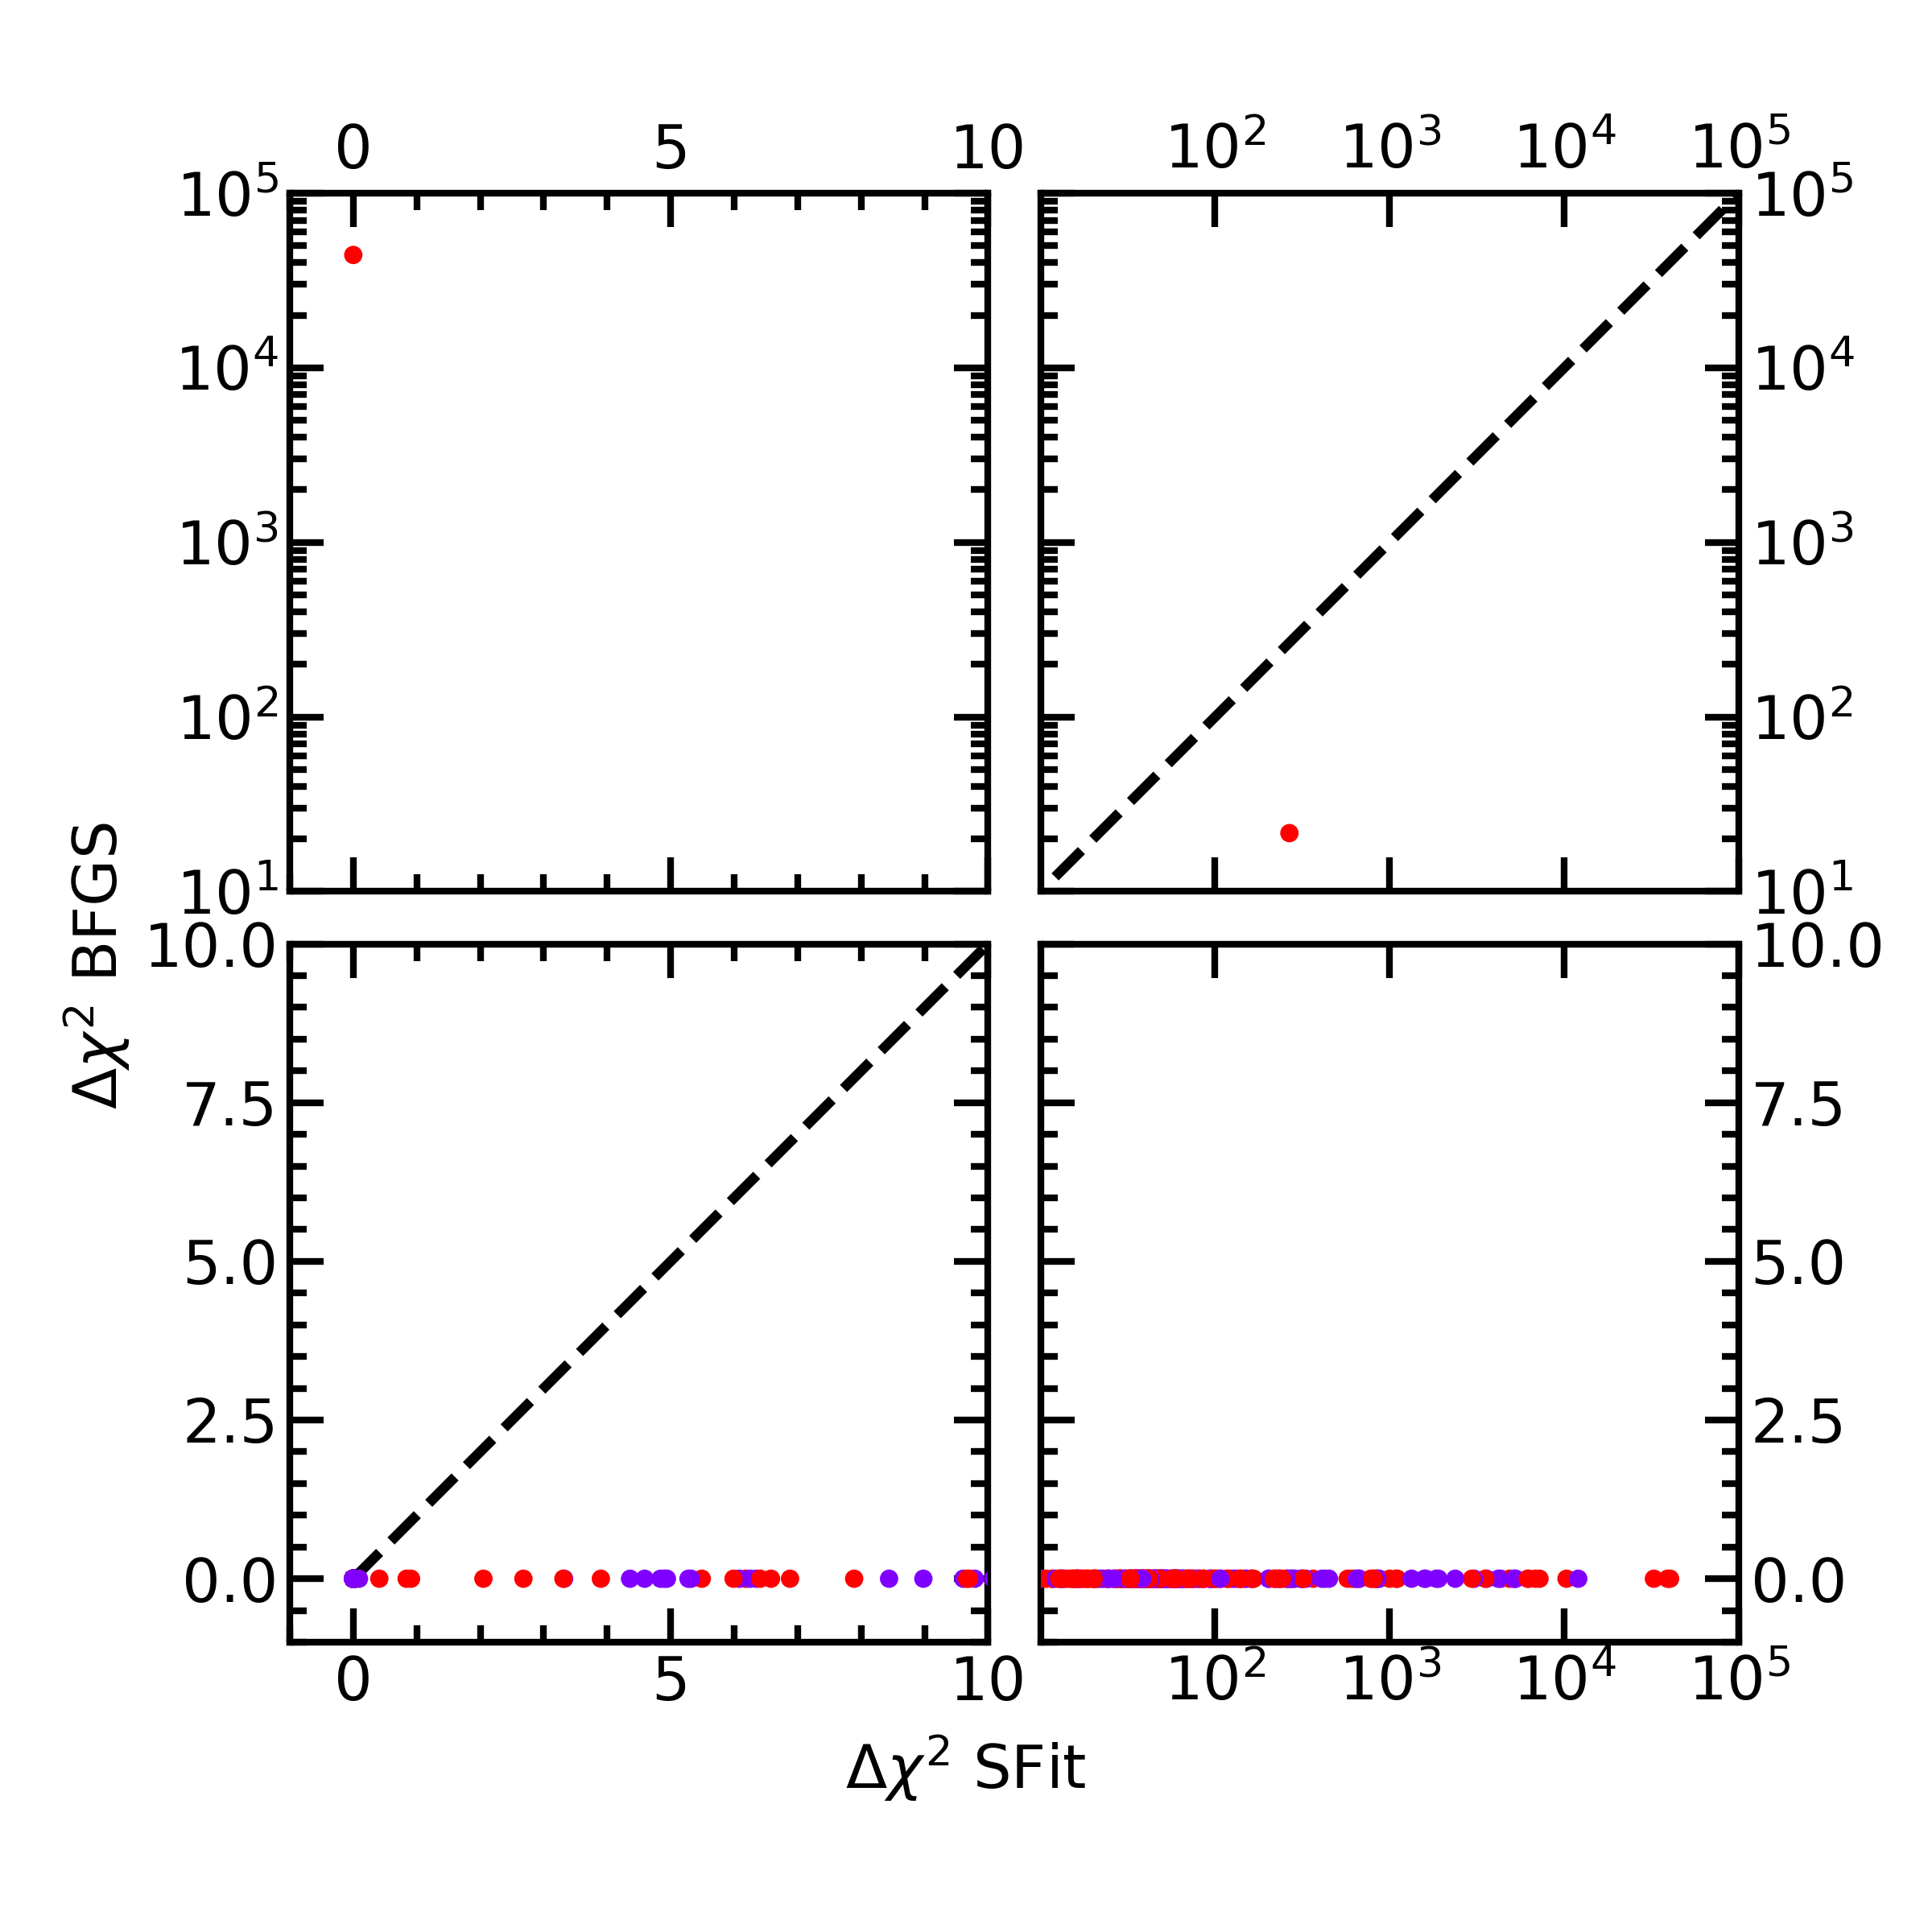
\includegraphics[width=0.33\textwidth]{figs/Dchi2_BFGS.png}
	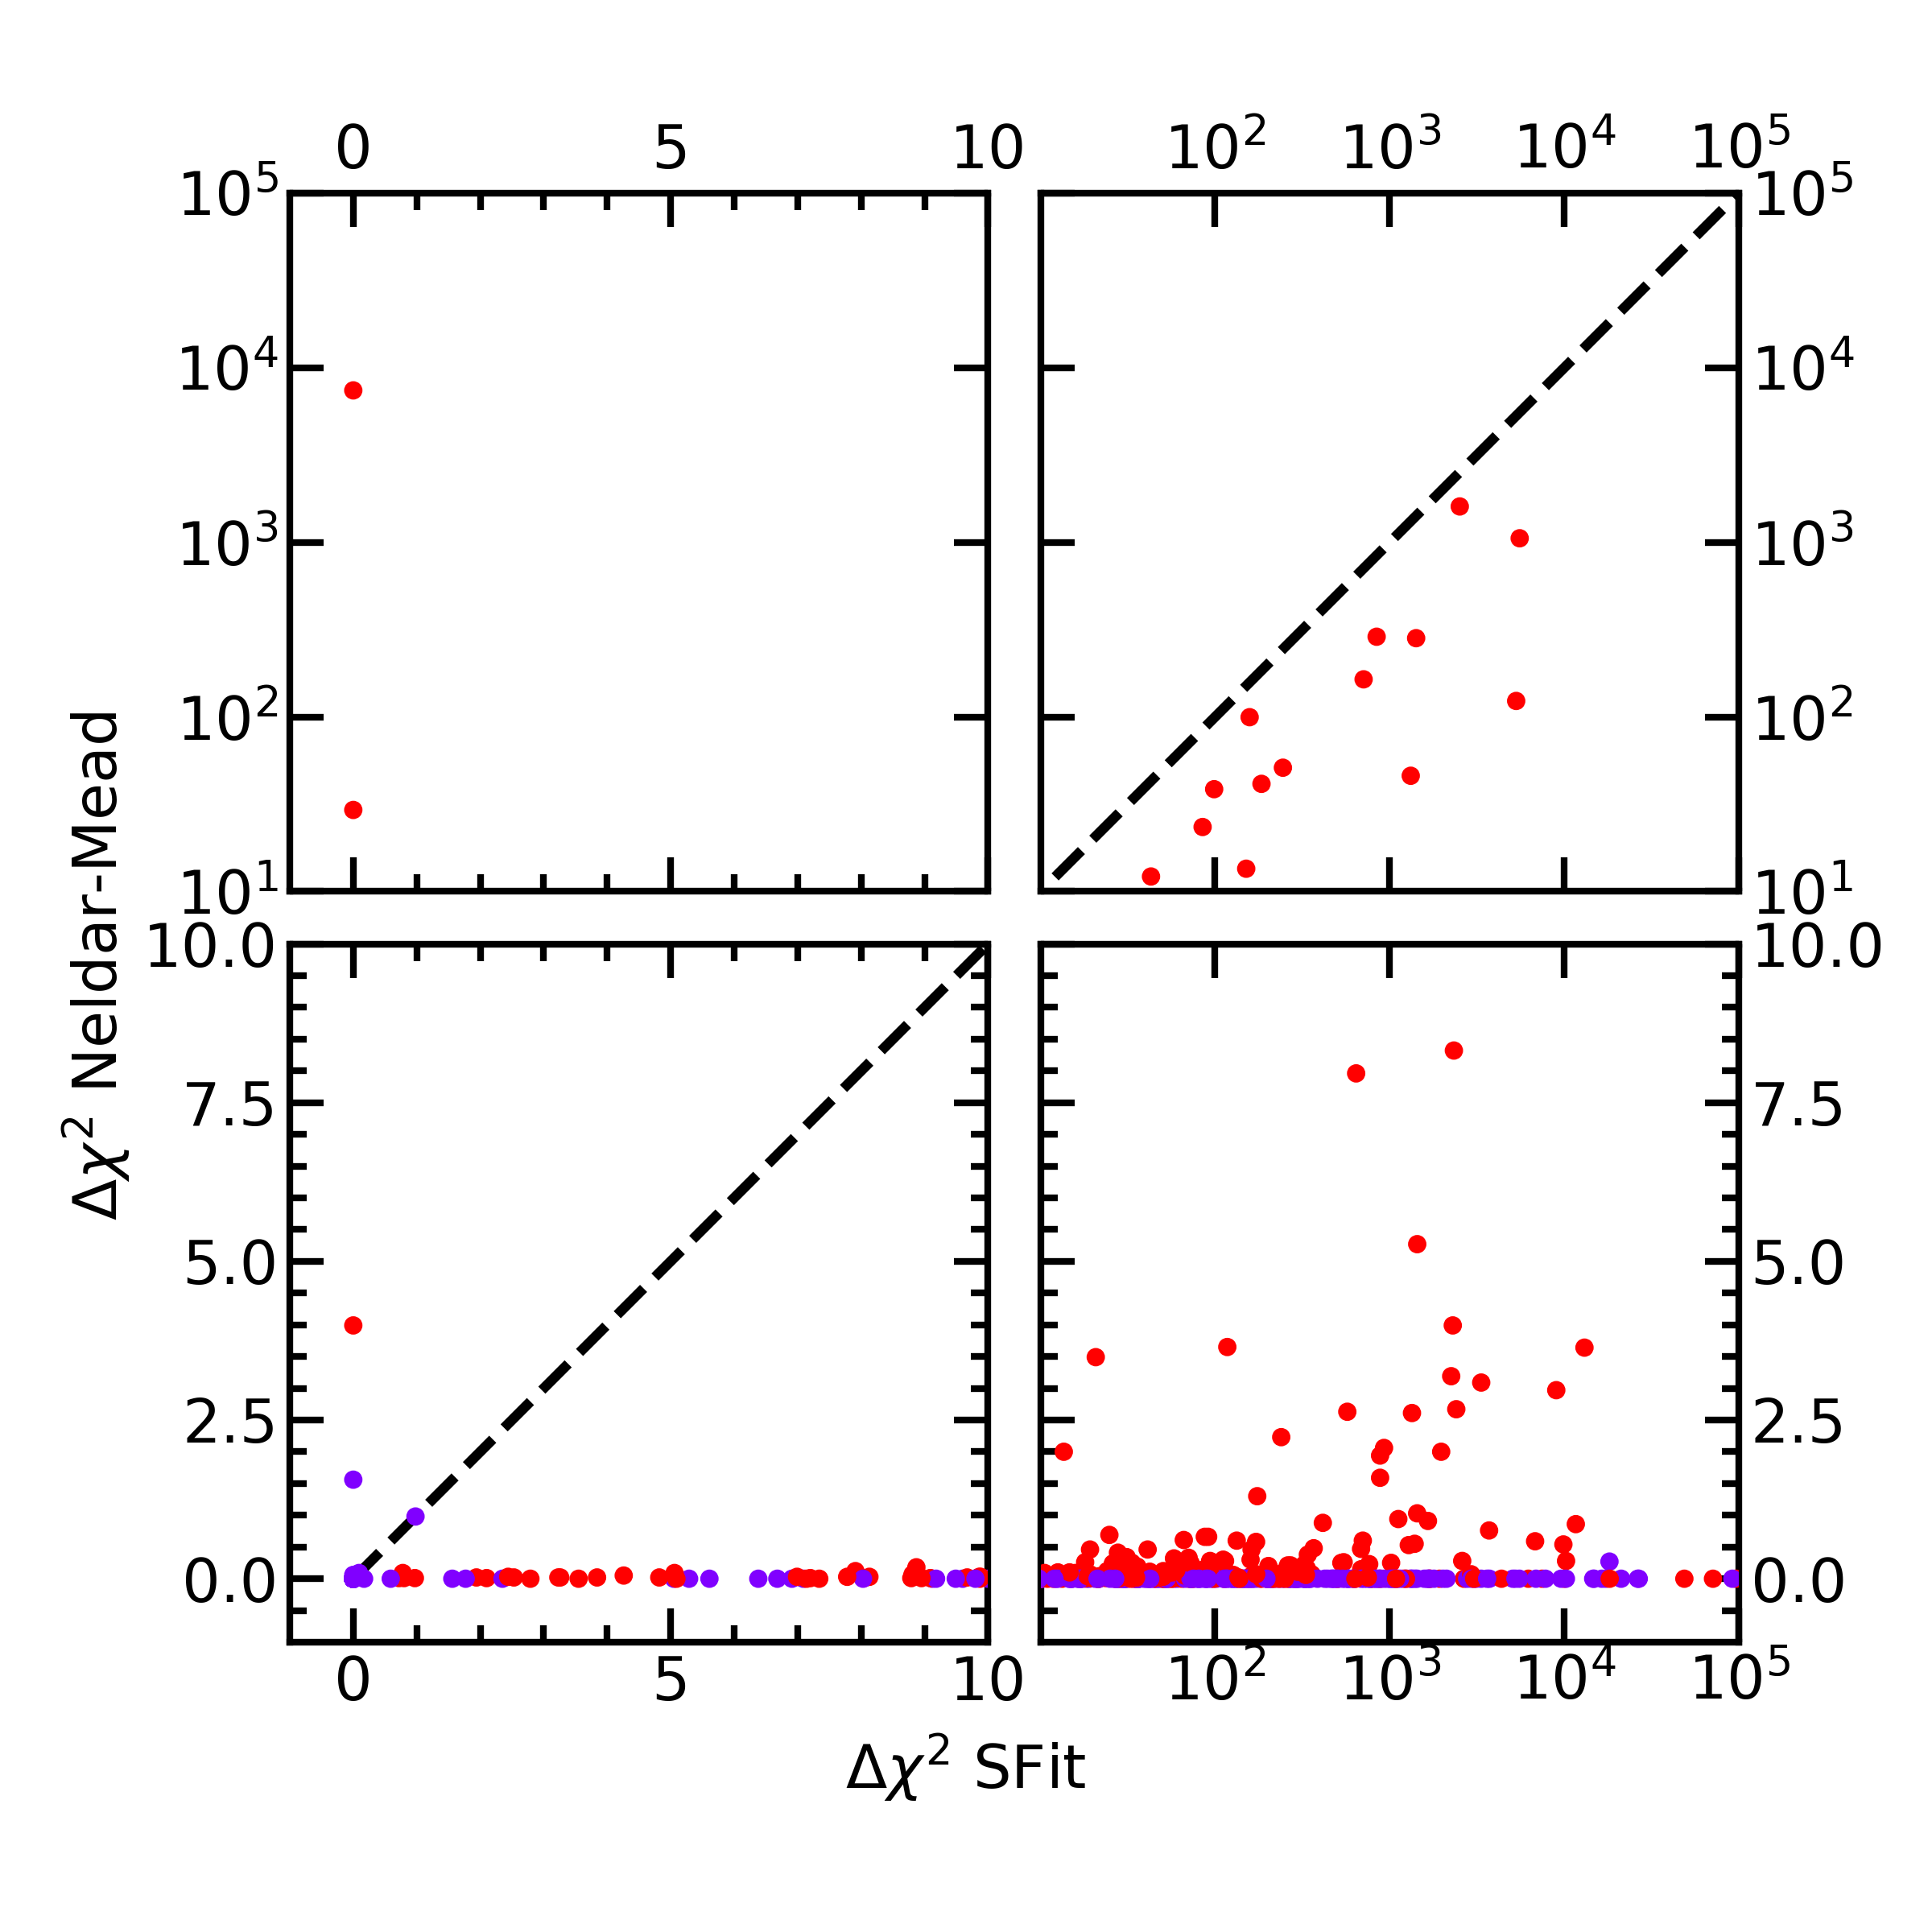
\includegraphics[width=0.33\textwidth]{figs/Dchi2_Neldar-Mead.png}
	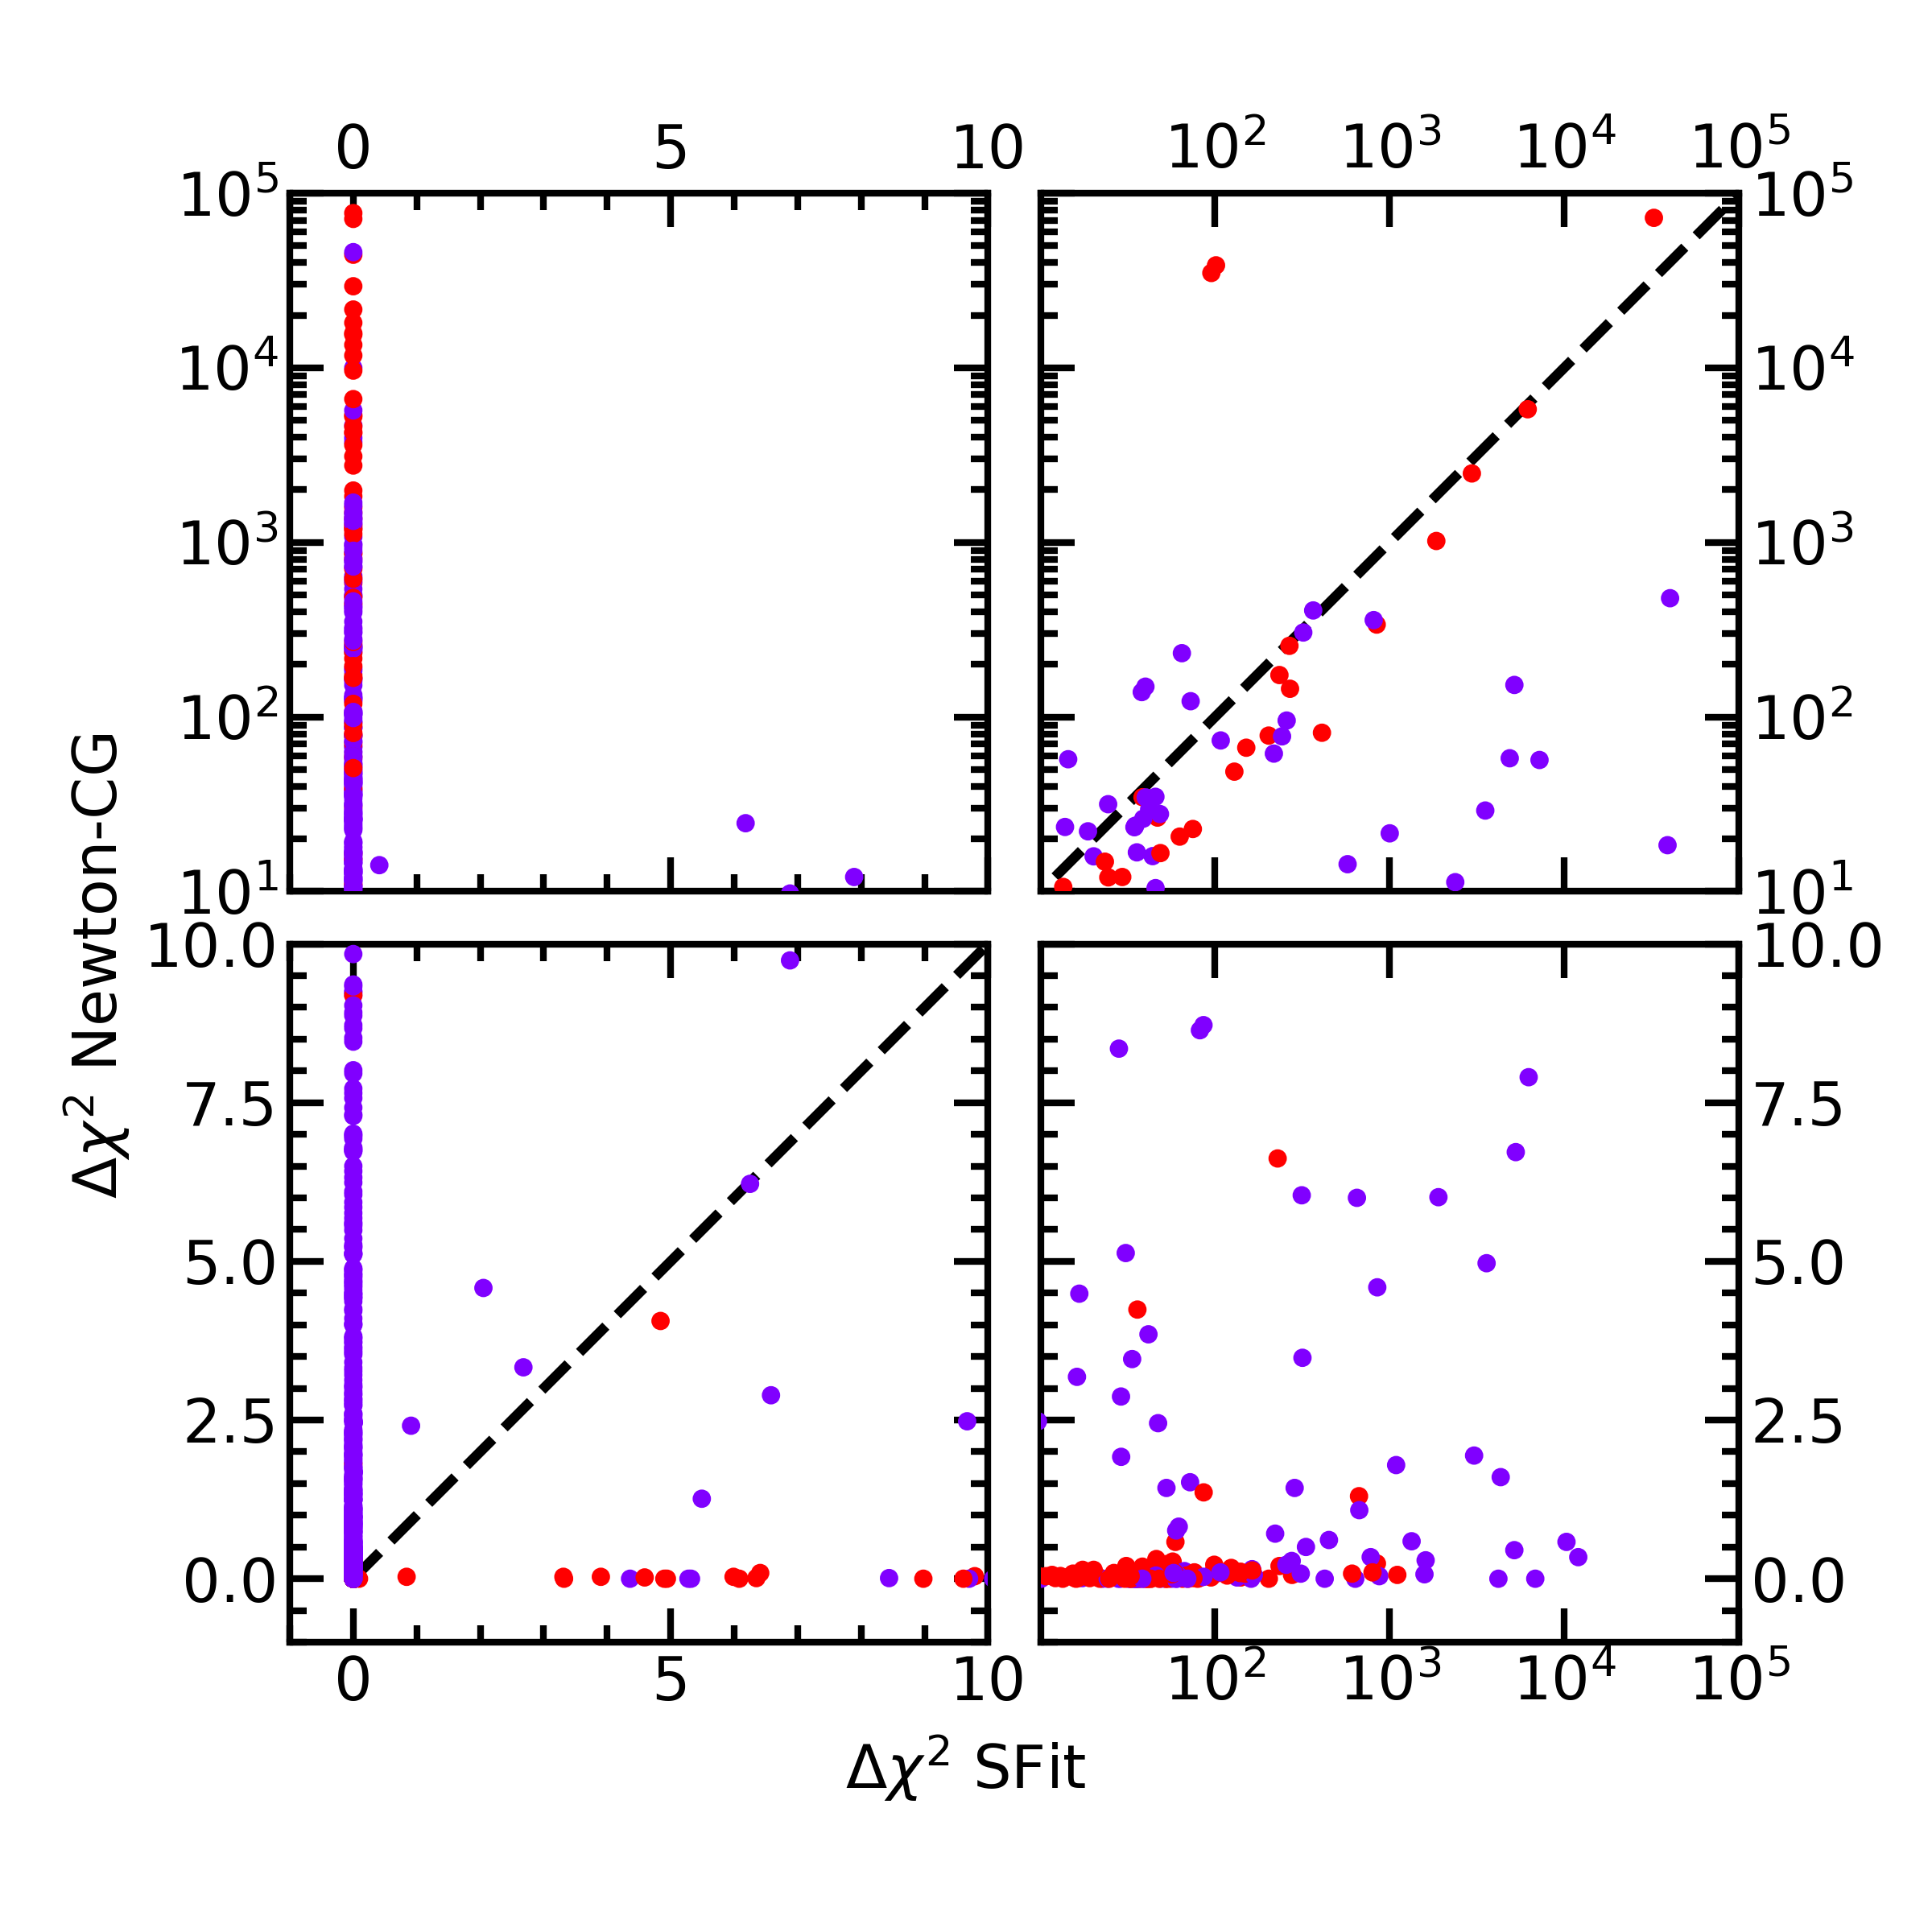
\includegraphics[width=0.33\textwidth]{figs/Dchi2_Newton-CG.png}
	\caption{$\Delta\chi^2$ relative to the best-fit for \bfgs, \neldarmead, and \newtoncg\, (the comparison algorithms)  vs. \sfit. Fits reported as successes by the comparison algorithm are plotted in purple, while those reported as failures are shown in red. Events that were fit successfully by both algorithms appear at (0, 0). In each set of four panels, the axes are split so that [0, 10] is on a linear scale, which [10, $10^5$] is on a log scale. The vertical bands of points at $x=0$ are fits that were successfully fit by \sfit\, but failed to be fit by the comparison algorithm; purple points in those bands are false positives for the comparison algorithm. The horizontal bands of points at $y=0$ are points for which the comparison algorithm successfully found the minimum but \sfit\, did not; red points in those bands are false negatives. 
	 \label{fig:dchi2}}
\end{figure}

\begin{deluxetable}{lr|rr|rr|rr|rr}
\tablecaption{Number of Fits with $\Delta\chi^2 \ge X$ of the Best-Fit}
\label{tab:dchi2}
\tablehead{
\colhead{} & \colhead{} & \multicolumn{4}{c}{$\Delta\chi^2 <$}\\
\colhead{Algorithm} & \colhead{Total} & \multicolumn{2}{|c}{0.1} & \multicolumn{2}{|c}{1.0} & \multicolumn{2}{|c}{10.0} & \multicolumn{2}{|c}{100.0} \\\colhead{} & \colhead{} & \multicolumn{1}{|c}{N} & \colhead{\%} & \multicolumn{1}{|c}{N} & \colhead{\%} & \multicolumn{1}{|c}{N} & \colhead{\%} & \multicolumn{1}{|c}{N} & \colhead{\%} 
}
\startdata
\hline\hline
\multicolumn{10}{l}{All 1822 Events:}\\
\hline\hline
\multicolumn{10}{l}{Algorithm Reported Success:}\\
\bfgs                 & 1074 & 1074 & 100 & 1074 & 100 & 1074 & 100 & 1074 & 100 \\
\neldarmead           & 1556 & 1551 & 100 & 1553 & 100 & 1554 & 100 & 1554 & 100 \\
\newtoncg             & 1630 &  572 &  35 &  727 &  45 &  888 &  54 & 1101 &  68 \\
\sfit                 & 1325 & 1324 & 100 & 1325 & 100 & 1325 & 100 & 1325 & 100 \\
\hline
\multicolumn{10}{l}{Algorithm Reported Failure:}\\
\bfgs                 &  748 &  722 &  97 &  725 &  97 &  727 &  97 &  728 &  97 \\
\neldarmead           &  266 &  155 &  58 &  225 &  85 &  247 &  93 &  256 &  96 \\
\newtoncg             &  192 &   65 &  34 &  111 &  58 &  125 &  65 &  137 &  71 \\
\sfit                 &  497 &    1 &   0 &    7 &   1 &   54 &  11 &  255 &  51 \\
\hline\hline
\multicolumn{10}{l}{1325 Events for which \sfit\, reported success:}\\
\hline\hline
\multicolumn{10}{l}{Algorithm Reported Success:}\\
\bfgs                 &  864 &  864 & 100 &  864 & 100 &  864 & 100 &  864 & 100 \\
\neldarmead           & 1321 & 1319 & 100 & 1320 & 100 & 1321 & 100 & 1321 & 100 \\
\newtoncg             & 1265 &  536 &  42 &  675 &  53 &  781 &  62 &  880 &  70 \\
\hline
\multicolumn{10}{l}{Algorithm Reported Failure:}\\
\bfgs                 &  461 &  455 &  99 &  456 &  99 &  457 &  99 &  458 &  99 \\
\neldarmead           &    4 &    1 &  25 &    1 &  25 &    2 &  50 &    3 &  75 \\
\newtoncg             &   60 &   27 &  45 &   28 &  47 &   29 &  48 &   34 &  57 \\
\hline\hline
\multicolumn{10}{l}{497 Events for which \sfit\, reported failure:}\\
\hline\hline
\multicolumn{10}{l}{Algorithm Reported Success:}\\
\bfgs                 &  210 &  210 & 100 &  210 & 100 &  210 & 100 &  210 & 100 \\
\neldarmead           &  235 &  232 &  99 &  233 &  99 &  233 &  99 &  233 &  99 \\
\newtoncg             &  365 &   36 &  10 &   52 &  14 &  107 &  29 &  221 &  61 \\
\hline
\multicolumn{10}{l}{Algorithm Reported Failure:}\\
\bfgs                 &  287 &  267 &  93 &  269 &  94 &  270 &  94 &  270 &  94 \\
\neldarmead           &  262 &  154 &  59 &  224 &  85 &  245 &  94 &  253 &  97 \\
\newtoncg             &  132 &   38 &  29 &   83 &  63 &   96 &  73 &  103 &  78 \\
\enddata
\end{deluxetable}


\begin{deluxetable}{lrrrr}
\tablecaption{Number of $\chi^2$ Function Evalutions}
\label{tab:nfev}
\tablehead{
\colhead{Algorithm} & \colhead{Mean} &  \colhead{Median} &  \colhead{StdDev} &  \colhead{Max\tablenotemark{a}}
}
\startdata
\bfgs                 & 122.1 &  44 & 217.2 & 830 \\
\neldarmead           & 348.8 & 303 & 136.6 & 603 \\
\newtoncg             &  44.5 &  21 &  80.2 & 633 \\
\sfit                 & 142.5 & 125 & 121.1 & 999\\
\enddata
\tablenotetext{a}{Fitting terminated after 999 function evaluations.}
\end{deluxetable}

\end{document}